% !TeX root =  main.tex

\section{Functions}


\begin{definition}[Function]

    A parabola is the set of all points in the plane that are equidistant from a fixed point $F$ (called the \textbf{focus}) and a fixed line $l$ (called the \textbf{directrix}).
\end{definition}
\begin{wrapfigure}[10]{r}{0.4\textwidth}
    \centering
    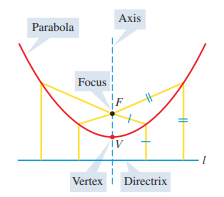
\includegraphics[width=0.3\textwidth,keepaspectratio]{figs/parabola-concepts.png}
\end{wrapfigure}
The \textbf{axis of symmetry} is the line that runs through the focus perpendicular to the directrix. The \textbf{vertex} $V$ is the intersection of the parabola and the axis of symmetry. Equivalently, the vertex lies halfway between the focus and the directrix.

\begin{theorem}[Parabola with vertical axis]
    A parabola has an equation $x^2=4py$ if and only if two of the following properties are satisfied:
    \begin{enumerate}[sepno]
        \item the vertex is $V(0, 0)$;
        \item the focus is $F(0, p)$;
        \item the directrix is $y=-p$.
    \end{enumerate}

    The parabola opens upward if $p>0$ or downward if $p<0$.
\end{theorem}

\begin{theorem}[Parabola with horizontal axis]
    A parabola has an equation $y^2=4px$ if and only if two of the following properties are satisfied:
    \begin{enumerate}[sepno]
        \item the vertex is $V(0, 0)$;
        \item the focus is $F(p, 0)$;
        \item the directrix is $x=-p$.
    \end{enumerate}

    The parabola opens to the right if $p>0$ or to the left if $p<0$.
\end{theorem}
\begin{center}
    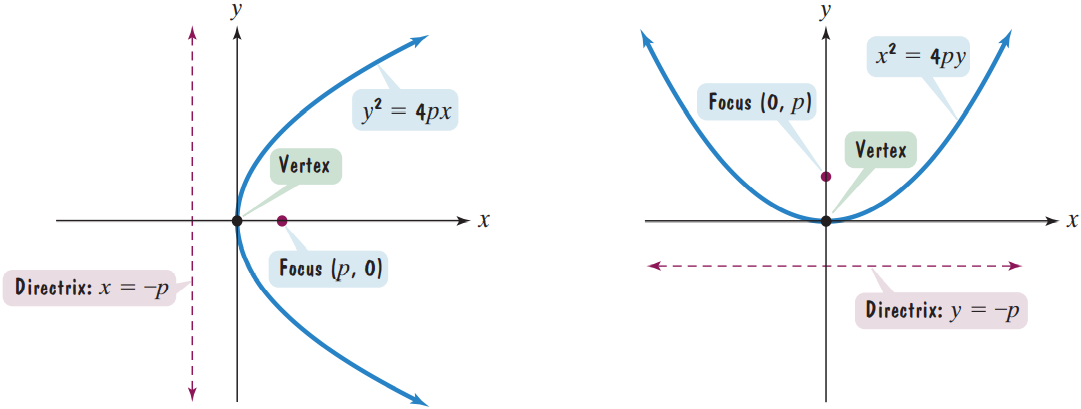
\includegraphics[width=0.8\textwidth,keepaspectratio]{figs/ParabolaGraphs.png}
\end{center}
The equations in the above theorems are called the standard form of the equation of a parabola with its vertex at the origin.

\begin{example}
    Find an equation of the parabola with the vertex $V(0,0)$ and focus $F(0,2)$.
\end{example}
\begin{solution}
    Because the vertex is $V(0, 0)$ and the focus is $F(0, 2)$. We know that $p=2$ and the axis of symmetry is vertical. Therefore, the parabola is defined by $x^2=8y$ by the theorem.
\end{solution}

\begin{example}
    Find the focus and directrix of the parabola $y=-x^2$.
\end{example}
\begin{solution}
    The equation of the parabola can be written as $x^2=-y$. Comparing with the standard form equation $x^2=4py$, we see that $4p=-1$ which implies $p=-\frac14$. So the focus is $\left(0, -\frac14\right)$ and the directrix is $y=-\left(-\frac14\right)$ which simplifies into $y=\frac{1}{4}$.
\end{solution}

The line segment that runs through the focus perpendicular to the
axis, with endpoints on the parabola, is called the \textbf{latus rectum}, and its length is the \textbf{focal diameter} of the parabola.

Because the latus rectum is parallel to the directrix and points on a parabola are equidistant from the focus and the directrix. The focal diameter equals the distance from the focus to the directrix. In particular, for a parabola with the vertex at the origin and the focus on a coordinate axis, the focal diameter is $|4p|$.

\begin{example}
    Find the focus, directrix, and focal diameter of the parabola $y=\frac{1}{2}x^2$.
\end{example}
\begin{solution}
    Rewriting the equation into standard form yields $x^2=2y$. Then $4p=2$ and $p=\frac{1}{2}$. Since the axis of symmetry is vertical, the focus is $(0, \frac12)$, the directrix is $y=-\frac12$, and the focal diameter is $|4p|=4\cdot\frac12=2$.
\end{solution}

\begin{example}
    A searchlight has a parabolic reflector that forms a “bowl,” which is 12 in. wide from rim to rim and 8 in. deep.  If the filament of the light bulb is located at the focus, how far from the vertex of the reflector is it?
\end{example}
\vspace{-2\baselineskip}
\begin{center}
    \noindent
    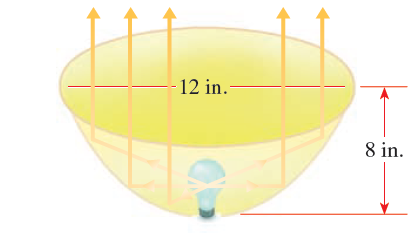
\includegraphics[height=8\baselineskip,keepaspectratio]{figs/SearchlightReflector1.png}
    \hspace{2em}
    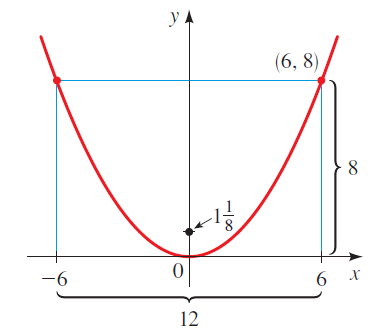
\includegraphics[height=9\baselineskip,keepaspectratio]{figs/SearchlightReflector2.png}
\end{center}

\begin{solution}
    We may assume the vertex is at the origin and the light bulb is at $F(0, p)$.
    Since the reflector is parabolic, that is the vertical section through the vertex and the light bulb is a parabola, an equation of the parabola is $x^2=4py$.
    Because the parabola is symmetric with respect to the axis of symmetry which is the vertical line passing through the vertex and the focus, there is a point $(6,8)$ on the parabola. It then follows that
    \[6^2=4p\cdot 8.\]
    Solving for $p$ yields $p=\frac{9}{8}$. So the light bulb is $\frac{9}{8}$ in. above the vertex of the reflector.
\end{solution}

\section{Ellipses}

\begin{definition}[Geometric Definition of an Ellipse]
    An \textbf{ellipse} is the set of all points in the plane the sum of whose distances from two fixed points $F_1$ and $F_2$ is a constant. These two fixed points are the \textbf{foci} (plural of focus) of the ellipse.
\end{definition}

\begin{definition}
    The midpoint of the line segment joining the foci is called the \textbf{center} of the ellipse.

    The line segment through the foci with endpoints on the ellipse is called the \textbf{major axis}

    The line segment perpendicular to the major axis through the center with endpoints on the ellipse is the \textbf{minor axis}.

    The intersections of the ellipse and the major axis are called the \textbf{vertices} of the ellipse.

    The distance of the foci to the center is called the \textbf{focal distance} or \textbf{linear eccentricity}.

\end{definition}

\begin{proposition}
    Suppose the length of the major axis is $2a$, the length of the minor axis is $2b$, and the linear eccentricity is $c$. Then
    \[a^2=b^2+c^2.\]
\end{proposition}

\begin{theorem}[Ellipse centered at the origin and with the major axis along the $x$-axis]
An ellipse has an equation $\frac{x^2}{a^2}+\frac{y^2}{b^2}=1$ if and only if the foci are $(\pm \sqrt{a^2-b^2}, 0)$ and the vertices are $(\pm a, 0)$, where $a>0$.
\end{theorem}

\begin{theorem}[Ellipse centered at the origin and with the major axis along the $y$-axis]
An ellipse has an equation $\frac{x^2}{b^2}+\frac{y^2}{a^2}=1$ if and only if the foci are $(0, \pm \sqrt{a^2-b^2})$ and the vertices are $(0, \pm a)$, where $a>0$.
\end{theorem}

\begin{center}
    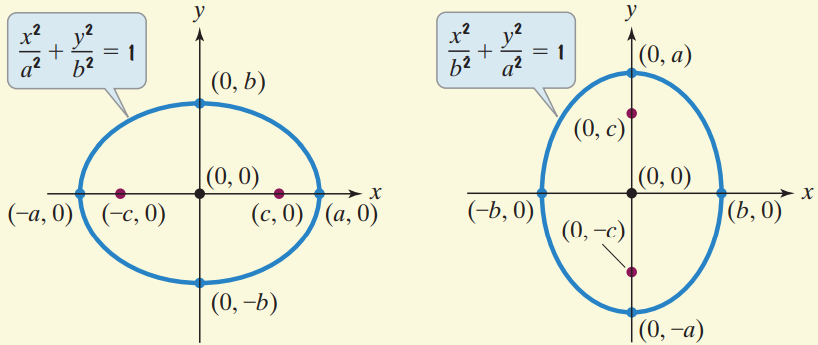
\includegraphics[width=0.8\textwidth,keepaspectratio]{figs/EllipseGraphs.png}
\end{center}

The questions of ellipses in the above theorems are called the \textbf{standard form}.

\begin{example}
    An ellipse has the equation $\dfrac{x^2}{9}+\dfrac{y^2}{4}=1$.
    Find the foci, the vertices, and the lengths of the major and minor axes. Sketch the graph.
\end{example}
\vspace*{6\baselineskip}

\begin{example}
    Find the foci of the ellipse $16x^2+9y^2=144$.
\end{example}
\vspace*{6\baselineskip}

\begin{example}
    Find an equation of the ellipse with the vertices $(\pm 4, 0)$ and the foci $(\pm 2, 0)$.
\end{example}
\vspace*{6\baselineskip}

\begin{definition}
    The eccentricity $e$ of an ellipse is defined as
    \[e=\dfrac{\text{focal distance}}{\frac12\left(\text{length of the major axis}\right)}.\]
    \begin{center}
        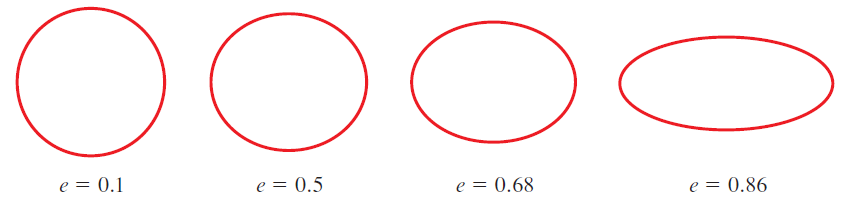
\includegraphics[scale=0.8]{figs/EllipseWithVariousEccentricities.png}
    \end{center}
\end{definition}

For an ellipse centered at the origin and with the major axis along a coordinate axis, the eccentricity is $e=\dfrac ca$.

\begin{example}
    Find the equation of the ellipse with foci $(0, \pm8)$ and the eccentricity $e=\frac45$.
\end{example}
\vspace*{8\baselineskip}

\section{Hyperbola}

\begin{definition}[Geometric Definition of a Hyperbola]
    A \textbf{hyperbola} is the set of all points in the plane, the difference of whose distances
    from two fixed points $F_1$ and $F_2$ is a constant. These two
    fixed points are the \textbf{foci} of the hyperbola.
\end{definition}

\begin{definition}
    The line segment containing the foci with endpoints on the hyperbola is called the \textbf{transverse axis}.

    The endpoints of the transverse axis are called the \textbf{vertices} of the hyperbola.

    The midpoint of the line segment joining the foci is the \textbf{center} of the hyperbola.

    The distance of the foci to the center is called the \textbf{focal distance} or \textbf{linear eccentricity}.

    The hyperbola consists of two separate curves, called \textbf{branches}, that are symmetric with respect to the transverse axis, conjugate
    axis, and center. \end{definition}


\begin{theorem}[Hyperbola centered at the origin and with the transverse axis along the $x$-axis]
A hyperbola has an equation $\frac{x^2}{a^2}-\frac{y^2}{b^2}=1$ if and only if the foci are $(\pm \sqrt{a^2+b^2}, 0)$ and the vertices are $(\pm a, 0)$.
\end{theorem}

\begin{theorem}[Hyperbola centered at the origin and with the transverse axis along the $y$-axis]
A hyperbola has an equation $\frac{x^2}{b^2}-\frac{y^2}{a^2}=1$ if and only if the foci are $(0, \pm \sqrt{a^2+b^2})$ and the vertices are $(0, \pm a)$.
\end{theorem}

\begin{center}
    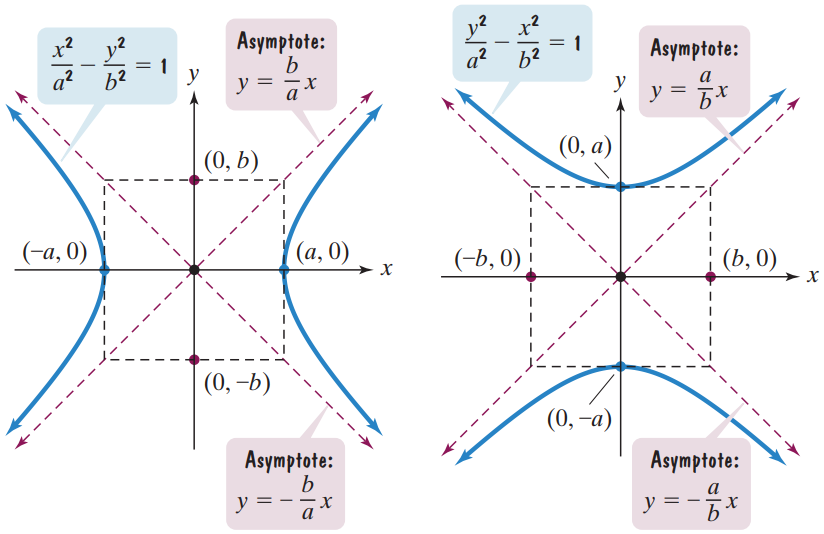
\includegraphics[width=0.8\textwidth,keepaspectratio]{figs/HyperbolaGraphs.png}
\end{center}

\begin{definition}
    A horizontal or oblique \textbf{asymptote} of a graph is a line with the property that the distance from the line to points on the graph approaches 0 as $x\to-\infty$ or as $x\to\infty$.
\end{definition}

A parabola has two asymptotes which are intersect at the center and symmetric with respect to the center or each axis.

\begin{proposition}[Characterization of hyperbola by asymptotes]
    A hyperbola has an equation $\dfrac{x^2}{a^2}-\dfrac{y^2}{b^2}=k$ if and only if its asymptotes are $y=\pm\dfrac{b}{a}x$ where $k$ is a non-zero real number.
\end{proposition}

The rectangle whose diagonals are along the aymptotes and with one side passing through a vertex of a hyperbola is called the \textbf{central box}.

The line segment through the center, perpendicular to the transverse axis with endpoints on the the central rectangle is the \textbf{conjugate axis}.

\begin{center}
    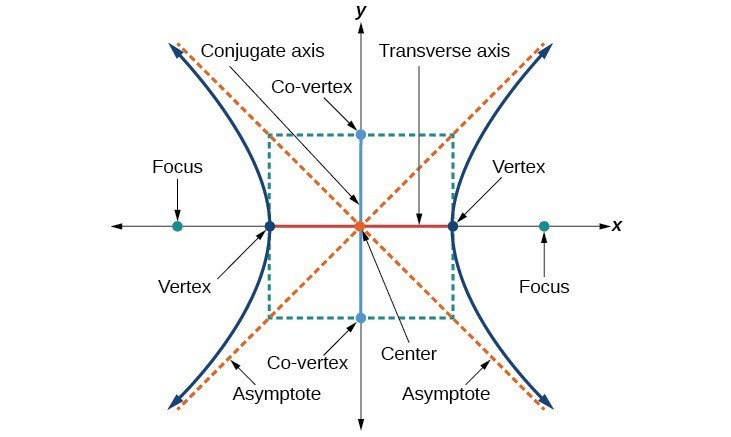
\includegraphics[width=0.7\textwidth,keepaspectratio]{figs/KeyConceptsOfHyperbola.jpg}
\end{center}

\begin{example}
    A hyperbola has the equation $9x^2-16y^2=121$.
    Find the vertices, foci, length of the transverse axis, and asymptotes. Sketch the graph.
\end{example}
\vspace*{8\baselineskip}

\begin{example}
    Find the vertices, foci, length of the transverse axis, and asymptotes of the hyperbola $x^2-9y^2+9=0$. Sketch the graph.
\end{example}
\vspace*{8\baselineskip}

\begin{example}
    Find the equation of the hyperbola with vertices $(\pm 3, 0)$ and foci $(\pm 4, 0)$.
\end{example}
\vspace*{8\baselineskip}

\begin{example}
    Find the equation and the foci of the hyperbola with vertices $(0,\pm 2)$ and asymptotes $y=\pm2x$.
\end{example}
\vspace*{8\baselineskip}

\section*{Practice}

\begin{exercise}
    Find the vertex, focus, and directrix of the parabola. Sketch the graph.\\
    \begin{enumerate*}
        \item $x^2=-8y$.
        \item $y^2=12x$.
        \item $x^2+6y=0$.
        \item $2x-y^2=0$.
    \end{enumerate*}
\end{exercise}
\vspace*{10\baselineskip}

\begin{exercise}
    An equation of an ellipse is given. Find the center, vertices, and foci of the ellipse, and the lengths of the major and minor axes. Sketch the graph.\\
    \begin{enumerate*}
        \item $\dfrac{x^2}{9}+\dfrac{y^2}{25}=1$.
        \item $\dfrac{y^2}{9}+\dfrac{x^2}{25}=1$.
        \item $9x^2+25y^2=1$.
        \item $25x^2+9y^2-16=0$.
    \end{enumerate*}
\end{exercise}
\vspace*{10\baselineskip}

\begin{exercise}
    An equation of an ellipse is given. Find the center, vertices, foci, and asymptotes of the hyperbola. Sketch the graph.\\
    \begin{enumerate*}
        \item $\dfrac{x^2}{9}-\dfrac{y^2}{25}=1$.
        \item $\dfrac{y^2}{9}-\dfrac{x^2}{25}=1$.
        \item $9x^2-25y^2=1$.
        \item $25x^2-9y^2-4=0$.
    \end{enumerate*}
\end{exercise}
\vspace*{10\baselineskip}

\begin{exercise}
    Find an equation for
    the conic section with the given properties.
    \begin{enumerate}
        \item The parabola with vertex at the origin and focus $(0, 5)$.
        \item The parabola with vertex at the origin and the directrix $x=-2$.
        \item The ellipse with vertices $(\pm 2, 0)$ and foci $(\pm 1, 0)$.
        \item the ellipse with foci $(0,\pm 3)$ and the eccentricity $e=\frac34$.
        \item The hyperbola with foci $(0,\pm 3)$ and vertices $(\pm 2, 0)$.
        \item The hyperbola with foci $(\pm 5, 0)$ and asymptotes $y=\pm\frac34$.
    \end{enumerate}
\end{exercise}

\begin{exercise}
    Find an question for the conic section with the given graph.
    \begin{enumerate}
        \item \mbox{}

        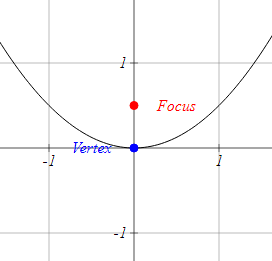
\includegraphics[width=0.3\textwidth]{figs/ParabolaEqFromGraph.png}
        \item \mbox{}

        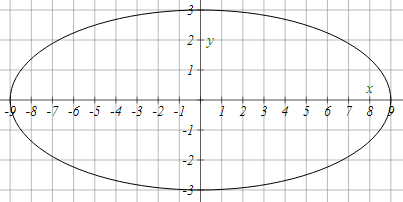
\includegraphics[width=0.4\textwidth]{figs/EllipseEqFromGraph.png}
        \item\mbox{}

        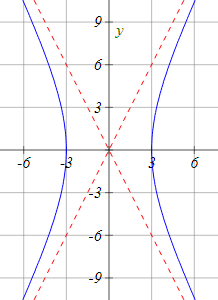
\includegraphics[width=0.3\textwidth]{figs/HyperbolaEqFromGraph.png}
    \end{enumerate}
\end{exercise}
